%%%%%%%%%%%%%%%%%%%%%%%%%%%%%%%%%%%%%%%%%%%%%%%%%%%%%%%%%%%%%%%%%%%%%%%%%%
% SignalsForwardConverterWithAsymHalfBridge
%%%%%%%%%%%%%%%%%%%%%%%%%%%%%%%%%%%%%%%%%%%%%%%%%%%%%%%%%%%%%%%%%%%%%%%%%%

\begin{solutionfigure}[htb]
    \centering
    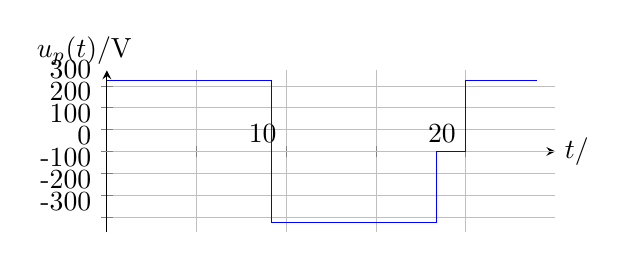
\begin{tikzpicture}
        \begin{axis}[
                domain=0:15,
                % x/y range adjustment
                xmin=0, xmax=25,
                ymin=-370, ymax=370,
                samples=250,
                axis y line=center,
                axis x line=middle,
                extra y ticks=0,
                % Label text
                xlabel={$t / \SI{}{\micro\second}$},,
                ylabel={$u_\text{p}(t)/\mathrm{V}$},
                % Label adjustment
                x label style={at={(axis description cs:1,0.5)},anchor=west},
                y label style={at={(axis description cs:-.05,.97)},anchor=south},
                width=0.6\textwidth,
                height=0.3\textwidth,
                % x-Ticks
                xtick={0,5,10,15,20},
                xticklabels={0,,10,,20},
                xticklabel style = {yshift=0.3cm,anchor=east},
                % y-Ticks
                ytick={300,200,100,-100,-200,-300},
                yticklabels={300,200,100,-100,-200,-300},
                yticklabel style = {yshift=0.2cm,anchor=east},
                % Grid layout
                grid=both,
                grid style={line width=.1pt, draw=gray!10},
                major grid style={line width=.2pt,draw=gray!50},
            ]
            \addplot[color=blue,mark=none,solid] coordinates{
                (0, 325)
                (9.2, 325)
                (9.2, -325)
                (18.4, -325)
                (18.4,0)
                (20, 0)
                (20, 325)
                (24, 325)
                };                
        \end{axis}     
    \end{tikzpicture}
    \caption{Voltage at primary side.}
    \label{fig:ex04_VoltageAtPrimarySide}
    \begin{tikzpicture}
        \begin{axis}[
                domain=0:15,
                % x/y range adjustment
                xmin=0, xmax=25,
                ymin=-2.2, ymax=3.5,
                samples=500,
                axis y line=center,
                axis x line=middle,
                extra y ticks=0,
                % Label text
                xlabel={$t / \SI{}{\micro\second}$},,
                ylabel={$i(t)/\mathrm{A}$},
                % Label adjustment
                x label style={at={(axis description cs:1,0.5)},anchor=west},
                y label style={at={(axis description cs:-.05,.97)},anchor=south},
                width=0.6\textwidth,
                height=0.3\textwidth,
                % x-Ticks
                xtick={0,5,10,15,20},
                xticklabels={0,,10,,20},
                xticklabel style = {yshift=0.3cm,anchor=east},
                % y-Ticks
                ytick={3,2,1,0,-1,-2},
                yticklabels={3,2,1,0,-1,-2},
                yticklabel style = {yshift=0.2cm,anchor=east},
                % Grid layout
                grid=both,
                grid style={line width=.1pt, draw=gray!10},
                major grid style={line width=.2pt,draw=gray!50},
            ]
            % im
            \addplot[color=red,mark=none,solid] coordinates{
                (0, 0)
                (9.2, 1.5)
                (18.4,0)
                (20, 0)
                (24,0.65)
                };      
            % Label of im
            \node[signalred, fill=white, inner sep = 1pt, anchor = south] at (axis cs:7,0.3) {$i_{\mathrm{m}}$};
            % i1
            \addplot[color=magenta,mark=none,solid] coordinates{
                (0, 0.3)
                (9.2, 2.2)
                (9.2, -1.5)
                (18.4,0)
                (20,  0.34)
                (24,1.28)
                };                
            % Label of i1
            \node[magenta, fill=white, inner sep = 1pt, anchor = south] at (axis cs:8,-1) {$i_{\mathrm{1}}$};
            % ip
            \addplot[color=black,mark=none,dashdotted] coordinates{
                (0, 0.34)
                (9.2, 2.24)
                (9.2, 1.54)
                (18.4,0.04)
                (20,  0.34)
                (24,1.32)
                };                
            % Label of ip
            \node[black, fill=white, inner sep = 1pt, anchor = south] at (axis cs:3,1.5) {$i_{\mathrm{p}}$};

            \end{axis}     
        \end{tikzpicture}
    \caption{Current at primary side.}    
    \label{fig:ex04_CurrentAtPrimarySide}
\end{solutionfigure}




